\documentclass[12pt]{article}

\usepackage[portuguese,linesnumbered,ruled,vlined]{algorithm2e}
\usepackage{sbc-template}
\usepackage{graphicx,url,amsfonts}

\usepackage[brazil]{babel}
\usepackage[utf8]{inputenc}
\usepackage{hyperref}

\pagenumbering{arabic}

\sloppy

\title{Trabalho Prático de Programação Natural\\Cubo Mágico}

\author{Gabriel de Biasi\inst{1}}

\address{
  Departamento de Ciência da Computação\\
  Universidade Federal de Minas Gerais\\
  Av. Antônio Carlos, 6627 -- Pampulha -- Belo Horizonte -- MG
  \email{biasi@dcc.ufmg.br}
}

\begin{document}

\maketitle

\section{Descrição do Problema}
  O brinquedo ``Cubo Mágico'' ou \textit{Rubik's Cube} foi criado por Ernő Rubik no ano de  1974 e distribuído comercialmente em 1980. Possui um conjunto de 26 cubos menores, 6 faces com três tipos de cubos distintos: São 4 centros, 12 meios e 8 quinas. Cada tipo cubo possui um número específico de cores, onde os centros possui uma cor, meios possuem duas cores e as quinas possuem três cores.

  É possível realizar movimentos em faces do cubo mágico sendo possível rotacionar os cubos desta face. Há 3 movimentos distintos que podem ser feitos em cada face, sendo eles: rotação horária, rotação anti-horária e dupla rotação. Logo, o cubo mágico tem um total de 18 movimentos possíveis.

  O objetivo principal deste jogo é fazer com que todas as faces tenham a mesma cor. Na \autoref{fig:cube} temos na esquerda um cubo em um estado ``bagunçado'' e outro no estado resolvido.

  \begin{figure}[!ht]
    \centering
    \caption{Cubo mágico bagunçado e um cubo mágico resolvido}
    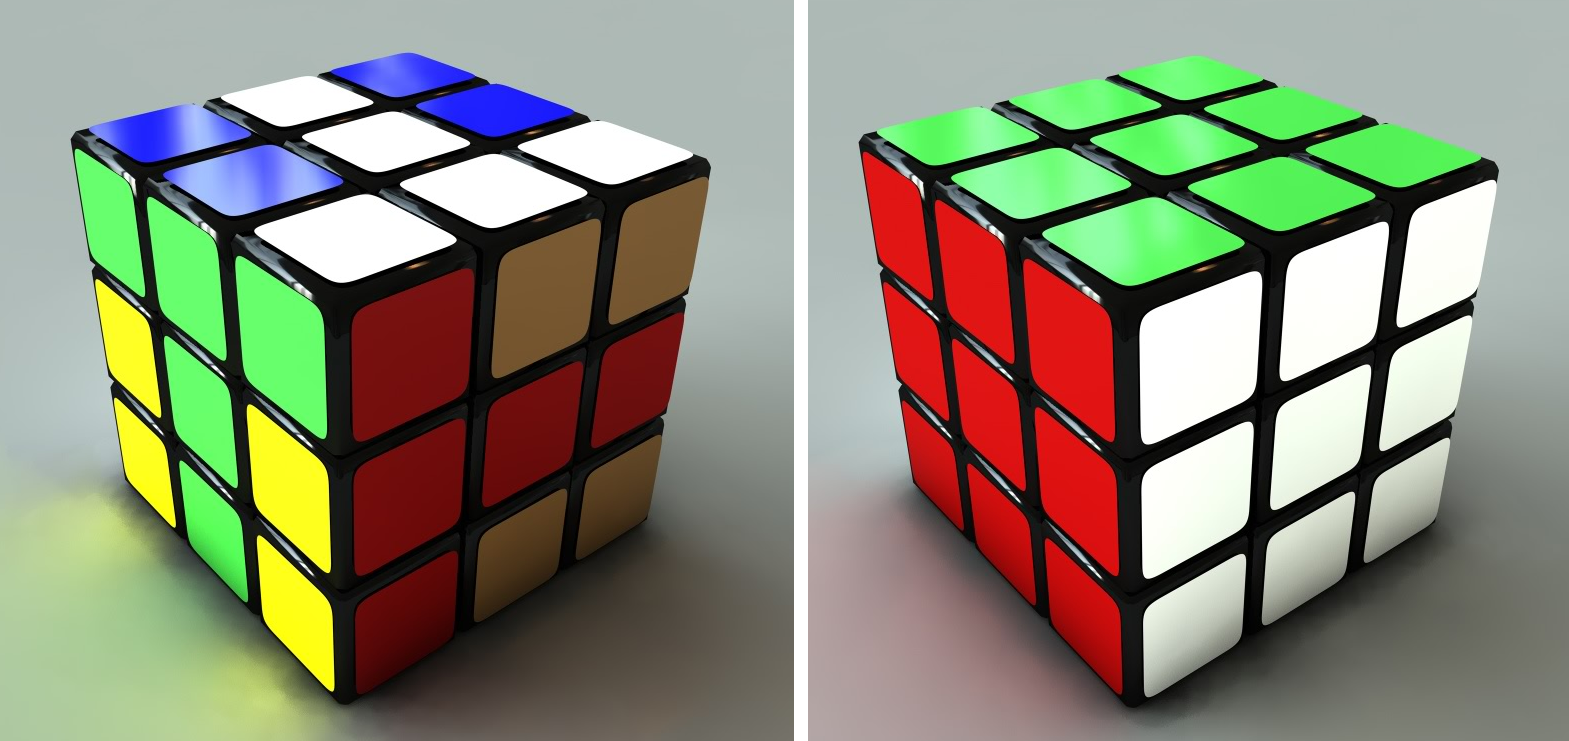
\includegraphics[scale=0.3]{images/cube.png}
    \label{fig:cube}
  \end{figure}

  O mapeamento dos movimentos possíveis no cubo mágico está de acordo com a \autoref{fig:moves}. Os movimentos horários nas faces da esquerda, direita, atrás, baixo, frente e topo serão, respectivamente, $L$, $R$, $B$, $D$, $F$ e $U$. Ao acrescentar a letra $i$, o movimento se torna anti-horário e ao acrescentar o número $2$, o movimento se tornará duplo.

  Foi provado matematicamente em 2010 que um cubo mágico em qualquer estado pode ser resolvido com 20 movimentos ou menos. Os cálculos foram realizados por um super computador fornecido pela Google. Detalhes sobre este projeto é encontrado no site do projeto: \url{http://www.cube20.org/}.

  \begin{figure}[!ht]
    \centering
    \caption{Movimentos do cubo mágico}
    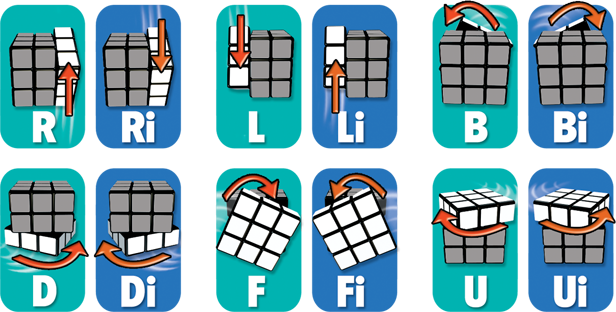
\includegraphics[scale=1.8]{images/moves.png}
    \label{fig:moves}
  \end{figure}

  Neste trabalho, é proposto um algoritmo evolutivo que tenha capacidade de resolver uma dada instância de cubo mágico colocando-o no estado resolvido e ao mesmo tempo buscando minimizar a quantidade de movimentos necessários.

\section{Metodologia}
  Para alcançar o objetivo do jogo, foi utilizado como base um método de resolução criado pelo professor \textit{Morwen Thistlethwaite}, onde o espaço de buscas de soluções é categorizado e então o cubo precisa ser levado de uma categoria para a próxima utilizando apenas os movimentos permitidos da categoria atual \cite{thistlethwaite}.

  \subsection{Categorias do Cubo}
    Thistlethwaite criou 5 categorias, que descreve o tão próximo um cubo mágico está da solução. As categorias diminuem drasticamente o espaço de busca de soluções, fazendo com que a busca pela solução simplifique com o avanço entre as categorias.

    \begin{description}
      \item [G0] Todos os estados do cubo mágico possíveis. Naturalmente, todos os cubos mágicos já estão presentes no conjunto G0. Sua ordem é de $|G0| = 4.33 \times 10^{19}$.
      \item [G1] Nesta categoria, os meios do cubo estão devidamente \textbf{orientados}, ou seja, não são permitidos os movimentos simples $[L, R]$ para colocá-los em sua posição original. Sua ordem é de $|G1| = 2.11 \times 10^{19}$.
      \item [G2] Na categoria G2 os meios da camada do meio não podem ser movidos de suas faces e a face de cima e a face de baixo só possuem suas respectivas cores amarelo/branco. Sua ordem é de $|G2| = 1.95 \times 10^{10}$.
      \item [G3] Todas as faces opostas do cubo mágico agora possuem suas determinadas cores. As faces frente/atrás terão laranja ou vermelho, cima/baixo terão amarelo ou branco e esquerda/direita terão verde ou azul. Sua ordem é de $|G3| = 6.63 \times 10^{5}$.
      \item [G4] Estado do cubo resolvido, $|G4| = 1$.
    \end{description}

  Os movimentos definidos por Thistlethwaite para cada categoria permitem levar para a próxima sem a quebra de propriedade. Este método de resolução facilita o estilo que um algoritmo evolutivo funciona, fazendo com que toda a população ganhe movimentos diferentes, entretanto, todos ainda pertencem à uma mesma categoria. Os movimentos permitidos são os descritos na \autoref{tab_mov}.

  \begin{table}[ht]
      \centering
      \caption{Movimentos permitidos em cada categoria} \label{tab_mov}
      \begin{tabular}{|c|c|}
        \hline
        \textbf{Categoria} & \textbf{Conjunto de Movimentos Permitidos}  \\ \hline
            G0             &  $(F, R, U, B, L, D)$           \\ \hline
            G1             &  $(F, R, U, B, L2, D2)$         \\ \hline
            G2             &  $(F, R, U2, B2, L2, D2)$       \\ \hline
            G3             &  $(F2, R2, U2, B2, L2, D2)$     \\ \hline
            G4             &  $\emptyset$                    \\ \hline
      \end{tabular}
  \end{table}


\section{Descrição Geral da Implementação}
  \cite{thistlethwaiteES} propuseram em seu artigo a utilização do método de Thistlethwaite porém com algumas modificações nas regras de movimentos e definição das funções de $fitness$.

  Neste trabalho, foi decidido manter os movimentos originais do trabalho de Thistlethwaite e as funções de $fitness$ e mutação precisaram ser adaptadas. A estrutura do algoritmo é explicada nas próximas subseções.

  \subsection{Fluxo de Trabalho do Algoritmo}
    O algoritmo inicia com a definição de três constantes, $Alpha\ (\alpha)$, $Theta\ (\Theta)$ e $Lambda\ (\lambda)$. Estas constantes representam, respectivamente, a quantidade de gerações máxima do algoritmo, o tamanho da população e a quantidade de indivíduos resolvidos necessária para avançar uma categoria.

    A população inicial de tamanho $\Theta$ é criada e todos os indivíduos estão vazios. Portanto, todos os indivíduos sofrem sua primeira mutação para iniciar as gerações.

    No início da geração, os indivíduos são ordenados por ranqueamento e os $\lambda$ melhores indivíduos são considerados os candidatos para a reprodução. Se todos os candidatos já pertecerem à próxima categoria, o algoritmo todo avança para a próxima categoria mudando o comportamento da função $fitness$ e de mutação. Todos os cadidatos possuem a mesma probabilidade de se reproduzirem e criar a próxima população, ao fim do processo, todos os novos indivíduos sofrem mutação e iniciam a próxima geração.

    O algoritmo encerra quando um indivíduo chega na categoria G4 ou quando o número de gerações definido por $\alpha$ for alcançado.

  \subsection{Definição de um Indivíduo}
    Neste algoritmo, um indivíduo é representado por uma simples lista de movimentos no cubo mágico, partindo do estado do cubo que foi passado quando o algoritmo iniciou.

    É importante ressaltar que cada indivíduo deste algoritmo evolucionário possui \textbf{quatro} valores de $fitness$ diferentes, que é melhor explicado na \autoref{fit}.
 
  \subsection{Seleção}
    A seleção de indivíduos é feita por ranqueamento simples, onde todos os todos indivíduos da população são ordenados pelo seu $fitness$ da categoria atual. Os $\lambda$ primeiros indivíduos são selecionados e considerados os candidatos para gerar a próxima população.

    Após a seleção, todos $\lambda$ candidatos terão a probabilidade $\frac{1}{\lambda}$ de serem escolhidos e então serem duplicados. Este processo se repete até que a nova população alcance a quantidade de $\Theta$ indivíduos.

  \subsection{Mutação}
    Ao criar a população inicial, todos os $\Theta$ indivíduos são vazios. O único processo que os modifica neste algoritmo é a mutação. De acordo com a categoria atual dos indivíduos da população, eles recebem uma sequência de movimentos diferentes. Ao iniciar uma mutação, é sorteado a quantidade de movimentos que serão concatenados, com uma quantidade mínima e máxima definida.

    Na \autoref{tab_mut}, está classificado a quantidade de movimentos que um indivíduo pode receber de acordo com cada categoria. Essas quantidades foram devidamente calculadas e definidas por Thistlethwaite.

    \begin{table}[ht]
      \centering
      \caption{Exemplos de Indivíduos} \label{tab_mut}
      \begin{tabular}{|c|c|}
        \hline
        \textbf{Categoria} & \textbf{Quantidade de Movimentos}  \\ \hline
            $G0\to G1$     &  $0 \leq l \leq 7$                 \\ \hline
            $G1\to G2$     &  $1 \leq l \leq 13$                \\ \hline
            $G2\to G3$     &  $2 \leq l \leq 15$                \\ \hline
            $G3\to G4$     &  $4 \leq l \leq 17$                \\ \hline
      \end{tabular}
    \end{table}

    Ao criar a nova sequência de movimentos, é provável que alguns movimentos possam ser removidos por serem complementares ou não produzir efeito final no cubo mágico. Portanto, todas as vezes que a mutação produz uma sequência de movimentos, ela é verificada pela função $clean$ em busca destes tipos de movimentos.

  \subsection{Função $clean$} \label{clean}
    Esta função é chamada toda vez que uma sequência de mutação é criada para um indivíduo. A fim de reduzir o número de movimentos necessários para resolver o cubo mágico, movimentos em sequência que não geram efeitos no cubo são removidos e movimentos que podem ser simplificados são alterados, sem perda de contexto final do cubo.
    
    A seguir, temos três exemplos de simplificação que podem ser feitos em uma sequência de movimentos. Na \autoref{tab_clean} apenas o movimento $F$ é apresentado, entretanto estas regras podem ser utilizadas para quaisquer movimentos do cubo mágico e em qualquer ordem.

    \begin{table}[ht]
      \centering
      \caption{Exemplos de Reduções de Movimentos} \label{tab_clean}
      \begin{tabular}{|c|c|c|}
        \hline
        \textbf{Inicial} & \textbf{Motivo}              & \textbf{Final}    \\ \hline
            $[F, Fi]$    &  Não produz efeito           &  $[\emptyset]$    \\ \hline
            $[F, F]$     &  Torna-se um giro duplo      &  $[F2]$           \\ \hline
            $[F, F2]$    &  Torna-se um giro invertido  &  $[Fi]$           \\ \hline
      \end{tabular}
    \end{table}

  \subsection{Função $fitness$} \label{fit}
    Para adequar-se ao estilo de categorias, foi necessário criar seis funções de $fitness$ diferentes, definidas como fases. O objetivo do algoritmo é \textbf{minimizar} os valores de $fitness$ de cada fase. Todos os valores terão o tamanho do indivíduo acrescentado à eles, portanto um indivíduo está resolvido para uma fase atual quando:

    \begin{equation}
    fitness\_fase_i = c
    \end{equation}

    Onde $c$ representa a quantidade de movimentos do indivíduo e $i$ representa a fase atual do algoritmo.

    Para fins de padronização, o cubo mágico deste algoritmo tem a face da frente com a cor laranja, face  de trás com a cor vermelha, face do topo com a cor amarela, face de baixo com a cor branca, face da esquerda com a cor verde e a face da direita com a cor azul.

    \subsubsection{Mudança de $G0 \to G1$}
      Neste momento, precisamos verificar se os movimentos dos indivíduos deixam o cubo no estado G1, onde os meios do cubo mágico estão orientados. Sendo $w$ o número de meios mal-orientados, a função de fitness é definida como:

      \begin{equation}
      fitness\_fase_0 = (10 \times w) + c
      \end{equation}

    \subsubsection{Mudança de $G1 \to G2$}
      Nesta fase os meios que pertencem à camada do meio precisam ser colocados em sua camada, porém não é necessário colocá-lo em seu local exato. Sendo $w$ o número de meios fora da camada do meio, a função de fitness é definida como:
      
      \begin{equation}
      fitness\_fase_1 = (10 \times w) + c
      \end{equation}

      Ainda na mesma categoria, agora nesta nova fase os cantos também precisam ser orientados. Sendo $v$ o número de cantos mal-orientados, a função de fitness é definida como:

      \begin{equation}
      fitness\_fase_2 = (40 \times v) + fitness\_fase_1
      \end{equation}

      Como as fases 1 e 2 são parte do mesmo grupo de movimentos, suas funções de $fitness$ foram separadas para melhor convergência porém no cálculo final são agregadas para garantir o mesmo resultado final.

    \subsubsection{Mudança de $G2 \to G3$}
      Os cubos na categoria G2 possuem suas faces topo e baixo com suas cores amarelo/branco. Agora, é necessário igualar as cores dos pares de cantos do cubo.

      Cada par de cantos do cubo mágico neste algoritmo é definido como o canto que está na camada do topo junto ao canto que está na camada de baixo, formando uma ``coluna'' no cubo mágico. Sendo $y$ o número de cada par de cantos incorretos, a função de $fitness$ é definida como:

      \begin{equation}
      fitness\_fase_3 = (5 \times y) + c
      \end{equation}

      Ainda nesta categoria, agora é preciso fazer que cada face do cubo tenha sua cor correta ou sua cor oposta. Sendo $x$ o número de cores erradas para todas as faces e $y$ o número de pares de cantos incorretos da fase anterior, a função de $fitness$ é definida como: 

      \begin{equation}
      fitness\_fase_4 = (5 \times (x + 2 \times y)) + c
      \end{equation}

      Como as fases 3 e 4 também fazem parte do mesmo grupo de movimentos, suas funções de $fitness$ também foram separadas, similar ao processo das fases 1 e 2.

    \subsubsection{Mudança de $G3 \to G4$}
      Neste ponto, todos os cubos estão na categoria G3 e possuem apenas cores corretas e cores opostas em suas faces. É necessário agora apenas os movimentos duplos para concluir o cubo mágico. Sendo $z$ o número de cores que não estão na sua face correta, a função de $fitness$ é definida como:

      \begin{equation}
      fitness\_fase_5 = (5 \times z) + c
      \end{equation}

      O algoritmo encerra ao primeiro indivíduo que obtiver a $fitness\_fase_5 = c$, pois
      pela ordenação da fase de seleção terá a menor quantidade de movimentos.

\section{Execução dos Experimentos}
  lala

\section{Conclusão}
  Neste trabalho.

\bibliographystyle{sbc}
\bibliography{ref}

\end{document}
